\documentclass{beamer}
\mode<presentation>{}
	\usepackage{hyperref}
	\usepackage{mathtools}
	\renewcommand{\vec}[1]{\mathbf{#1}}
	\graphicspath{{Figures/}}
	\usetheme{CambridgeUS}

\AtBeginSection[]{
{
  \setbeamertemplate{footline}{}
  \begin{frame}[noframenumbering]
  \vfill
  \centering
  \begin{beamercolorbox}[sep=8pt,center,shadow=true,rounded=true]{title}
    \usebeamerfont{title}\insertsectionhead\par
  \end{beamercolorbox}
  \vfill
  \end{frame}
}
}

\AtBeginSubsection[]{
{
  \setbeamertemplate{footline}{}
  \begin{frame}[noframenumbering]
  \vfill
  \centering
  \begin{beamercolorbox}[sep=8pt,center,shadow=true,rounded=true]{title}
    \usebeamerfont{title}\insertsubsectionhead\par
  \end{beamercolorbox}
  \vfill
  \end{frame}
}
}

\setlength{\abovedisplayskip}{3pt}
\setbeamertemplate{navigation symbols}{}
\setbeamertemplate{footline}{
\leavevmode
\hbox{
\begin{beamercolorbox}[wd=\paperwidth,ht=2.25ex,dp=1ex,right]{}
   \insertframenumber{} \hspace*{2ex} 
  \end{beamercolorbox}
}
\vskip0pt
}
\makeatother

\title{Long-term Conservation of Geometric Invariants by Newmark Beta methods}
\subtitle{Numerical Computation Structured Projects}
\date{Hilary Term, 2018}

\begin{document}

{
\setbeamertemplate{footline}{}
\begin{frame}[noframenumbering]
	\titlepage
\end{frame}
}

\section{Introduction}
\begin{frame}{Geometric Numerical Integration Timeline}
	\begin{itemize}
		\item<1->
			Relatively young field - came into limelight around 40 years ago
		\item<1->
			Study of numerical solutions to ordinary differential equations had begun in the late 19\textsuperscript{th} Century
		\item<1->
			The focus had been on quantity - making the solutions as accurate as possible
		\item<1->
			Interest in computer simulations over a longer time frame raised an important question
	\end{itemize}
	\uncover<2-> {\centering \alert{What about the quality of solutions?}}
\end{frame}

\begin{frame}[t]{Newmark Beta methods}
\begin{align*}
		\vec{v}_{i+1} & = \vec{v}_{i} + h\left[\left(1-\gamma \right)\vec{a}_{i} + \gamma \vec{a}_{i+1}\right], \\
		\vec{x}_{i+1} & = \vec{x}_{i} + h\vec{v}_{i} + \frac{h^2}{2}\left[ \left(1-2\beta \right)\vec{a}_{i} + 2\beta \vec{a}_{i+1}\right] ,
\end{align*} where $\gamma \in \left[0, 1 \right]$ and $\beta \in \left[0, \frac{1}{2} \right]$.
\bigskip
\begin{itemize}
	\item
	Implicit if $\beta > 0$
	\item
	Explicit If $\beta = 0$ and acceleration depends only on displacement
	\item 
	Second order accurate $\Leftrightarrow \gamma = \frac{1}{2}$
\end{itemize}
\end{frame}

\begin{frame}{Computational Application of Newmark Beta methods}
\only<1-1> {
	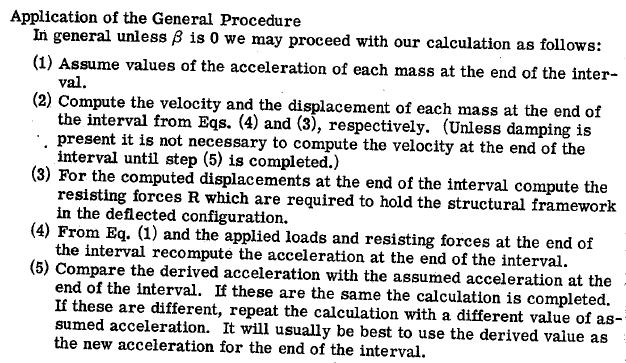
\includegraphics[width=\textwidth, angle=1]{newmark-beta_algorithm_original}
}
\only<2-2> {
	\begin{align*}
			\vec{v}_{i+1} & = \vec{v}_{i} + h\left[\left(1-\gamma\right)\vec{a}_{i} + \gamma\vec{a}_{i+1}\left(\vec{x}_{i+1}\right)\right], \\
			\vec{x}_{i+1} & = \vec{x}_{i} + h\vec{v}_{i} + \frac{h^2}{2}\left[\left(1-2\beta \right)\vec{a}_{i} + 2\beta\vec{a}_{i+1}\left(\vec{x}_{i+1}\right)\right]. 
	\end{align*}
	\dotfill
	\medskip
	\begin{align*}
		\vec{\tilde{F}}\left(\vec{x}_{i+1}\right) & = \vec{x}_{i+1} - \vec{x}_{i} -h\vec{v}_{i} - \frac{h^{2}}{2}\left[\left(1-2\beta\right)\vec{a}_{i} + 2\beta\vec{a}_{i+1}\left(\vec{x}_{i+1}\right)\right], \nonumber \\
		D_{\vec{x}_{i+1}}\vec{\tilde{F}}\left(\vec{x}_{i+1}\right) & = \textbf{I} -  \beta h^{2}\textbf{J}_{\vec{a}_{i+1}},\nonumber \\
		\vec{x}_{i+1} & = \vec{x}_{i} - D\vec{\tilde{F}}\left(\vec{x}_{i}\right)^{-1}\vec{\tilde{F}}\left(\vec{x}_{i}\right).
	\end{align*}
}
\end{frame}

\section{Molecular Dynamics}

\begin{frame}{Hamiltonian System}
We have to solve the Hamiltonian
\medskip
\begin{align*}
	H(p, q) = \frac{1}{2}\sum_{i = 1}^{N} m_{i}^{-1}p_{i}^{T}p_{i} + \sum_{i=1}^{N-1} \sum_{j=i+1}^{N} V\left(\left\Vert q_{i} - q_{j} \right\Vert_{2}\right).
\end{align*}
\end{frame}

\begin{frame}{Lennard-Jones Potential}
\begin{columns}
	\column{0.5\textwidth}
	\begin{align*}
		V\left(\vec{r}_{ij}\right) = 4\varepsilon \left[ \left( \frac{\sigma}{r_{ij}}\right)^{12} - \left( \frac{\sigma}{r_{ij}}\right)^{6} \right],
	\end{align*}

	\column{0.5\textwidth}
	\centering
	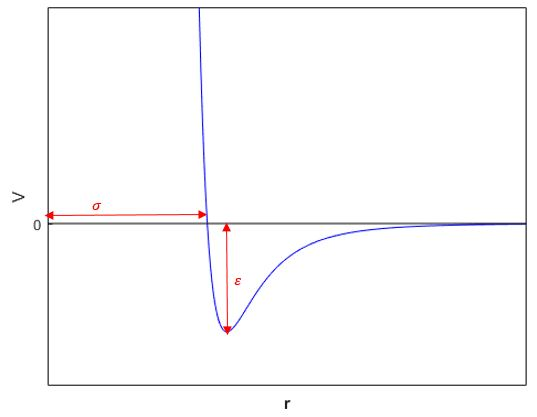
\includegraphics[scale=0.40]{lennard-jones_potential_graph}
\end{columns}
where
$$
\arraycolsep=2pt
\begin{array}{rl}
	\vec{r}_{ij} &\mbox{is the displacement between the $i^{th}$ and the $j^{th}$ atoms} \\
	r_{ij} &= \left\Vert\vec{r}_{ij}\right\Vert_{2} \\
	\varepsilon & \mbox{is the potential well depth} \\
	\sigma & \mbox{is the distance at which the potential between two atoms is 0}
\end{array}
$$
\end{frame}

\begin{frame}[t]{Simulation Details}
\only<1-1> {
\begin{itemize}
	\item Initial Positions: cube of 864 particles at a density of $1.374 \mbox{ g}\cdot\mbox{cm}^{-3}$
\end{itemize}
\begin{figure}
	\centering
	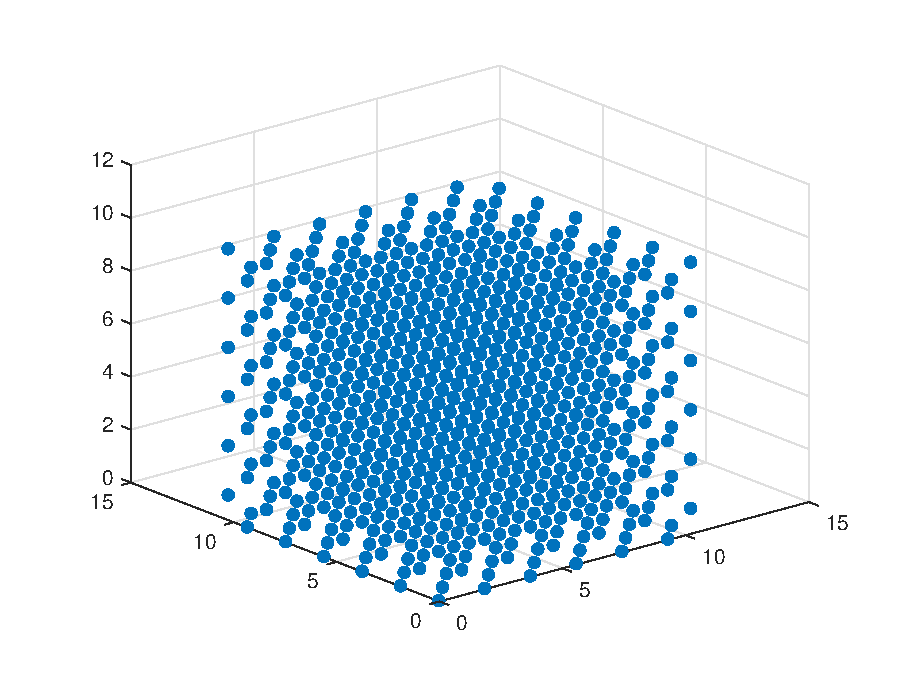
\includegraphics[scale=0.5]{fcc_lattice_-40_25.eps}
	\caption{Face-centered cubic lattice of  864 particles at a density of $1.374 \mbox{ g}\cdot\mbox{cm}^{-3}$}
\end{figure}
}

\only<2-2> {
\begin{itemize}
	\item Initial Velocities: Maxwellian distribution of velocities
\end{itemize}
\vfill
\begin{align*}
	f_{\vec{v}}\left(v_{x}, v_{y}, v_{z}\right) &= \left(\frac{m}{2\pi k_{B} T}\right)^{\frac{3}{2}}\exp\left[-\frac{m\left(v_{x}^{2}+v_{y}^{2}+v_{z}^{2}\right)}{2k_{B}T}\right]. \\
 	\mbox{So, } v_{x}, v_{y}, v_{z} &\sim \mathcal{N}\left(0,\frac{k_{B}T}{m}\right)
\end{align*}
\vfill
}

\only<3-3>{
\begin{itemize}
	\item Equilibration
\end{itemize}
\begin{figure}
	\centering
 	\begin{tabular}{@{}cc@{}}
		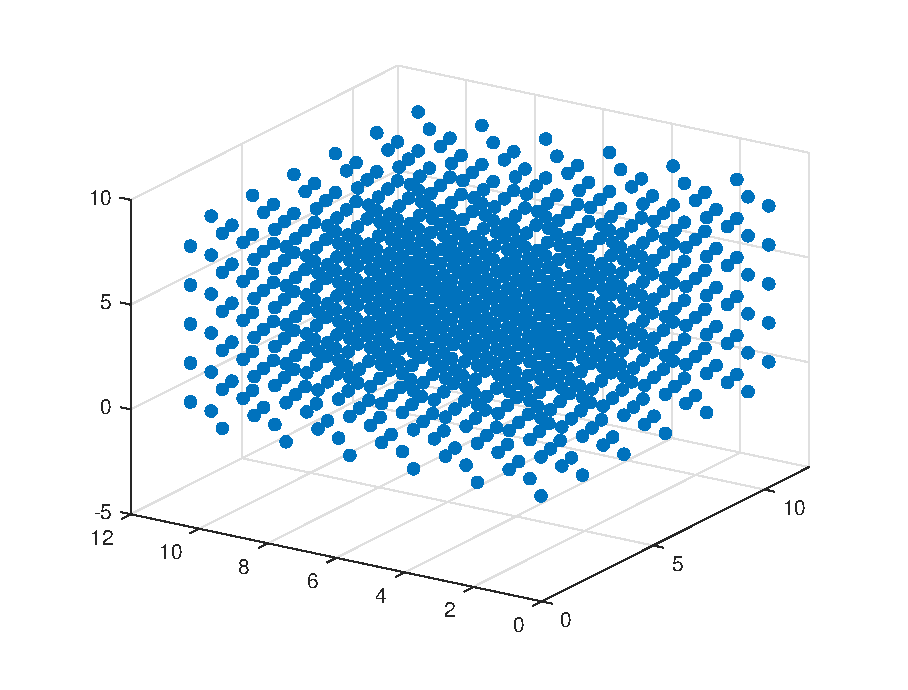
\includegraphics[width=0.5\textwidth]{initial_solid_-57_27_2.eps} &
  		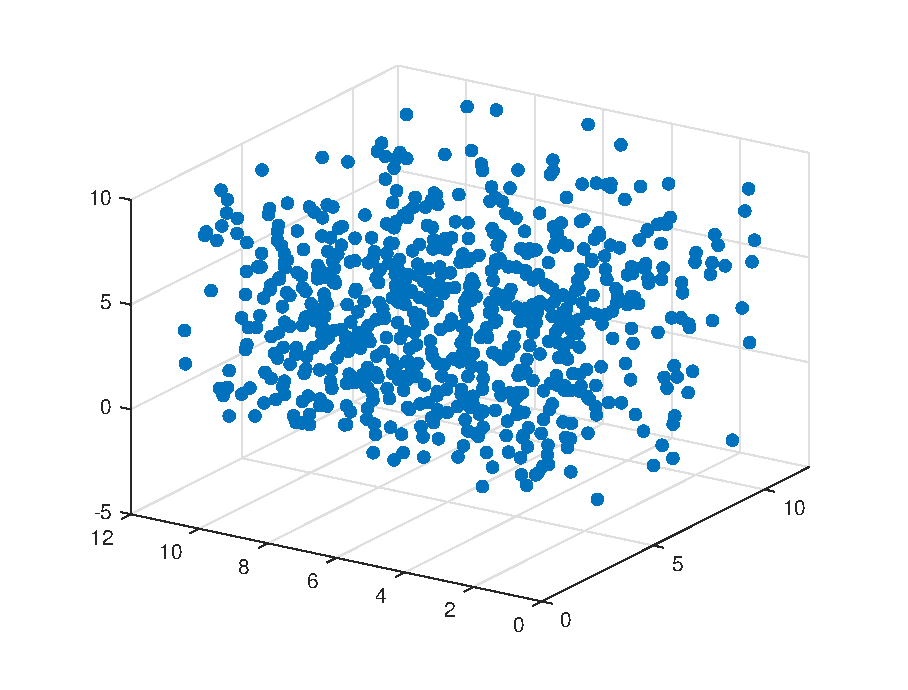
\includegraphics[width=0.5\textwidth]{equilibrated_solid_-57_27_2.eps} \\
 	\end{tabular}
  	\caption{Change in the position of particles after 500 steps of equilibration}
\end{figure}
}

\only<4-4>{
\begin{itemize}
	\item Periodic Boundary Conditions
\end{itemize}
\begin{figure}
	\centering
	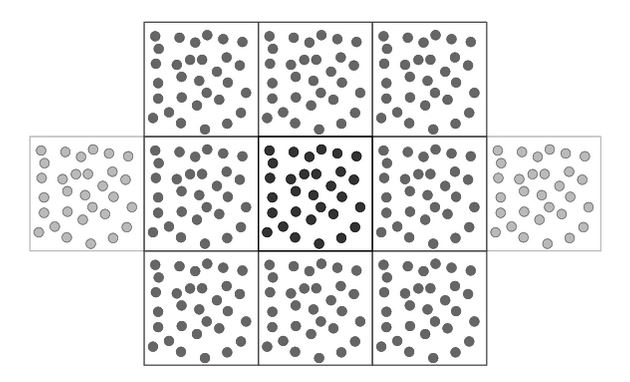
\includegraphics[scale=0.6]{periodic_boundary_condition_2d.jpg}
  	\caption{Periodic Boundary Conditons in 2-d}
\end{figure}
}
\end{frame}

\section{Conservation of Geometric Invariants}

\subsection{Time Reversibility}

\begin{frame}{Time Reversibility}
\begin{theorem} A Hamiltonian system is time reversible. \end{theorem}
\begin{proof}
	We apply the transformation $t \mapsto -t$.
	\begin{align*}
		q \mapsto q = \tilde{q},  \quad \quad p \mapsto -p = \tilde{p}.
	\end{align*}
	Then
	\begin{alignat*}{4}
		\dot{\tilde{q}} &= \frac{d\tilde{q}}{d\left(-t\right)} \quad &&= -\nabla_{\tilde{p}}H \quad &&= \nabla_{p}H \quad &&= \dot{q},\\
		\dot{\tilde{p}} &= \frac{d\tilde{p}}{d\left(-t\right)} \quad &&= -\nabla_{\tilde{q}}H \quad && =-\nabla_{q}H \quad &&= \dot{p}. \qedhere
	\end{alignat*}
\end{proof}
\end{frame}

\begin{frame}{Time Reversibility}
\begin{itemize}
	\item
	A numerical one-step method $\Phi_{h}: (\vec{x}_{i},\vec{v}_{i}) \mapsto (\vec{x}_{i+1},\vec{v}_{i+1})$ is time reversible if $\Phi_{h} = \Phi_{-h}^{-1}$.
	\item
	Informally, this means that if we exchange $i \leftrightarrow i+1$ and replace $h$ by $-h$ in our original method, then we should get the same method back.
	\item
	Any Newmark Beta method with $\gamma = \frac{1}{2}$  is reversible.
	\item	
	No other Newmark Beta method is reversible.
	\item
	However, rounding-off errors in practice mean that we may not get back the initial state of the system after reversing the velocities.
\end{itemize}
\end{frame}

\begin{frame}{Time Reversibility}
\only<1-1> {
	\begin{figure}
		\centering
 		\begin{tabular}{@{}cc@{}}
			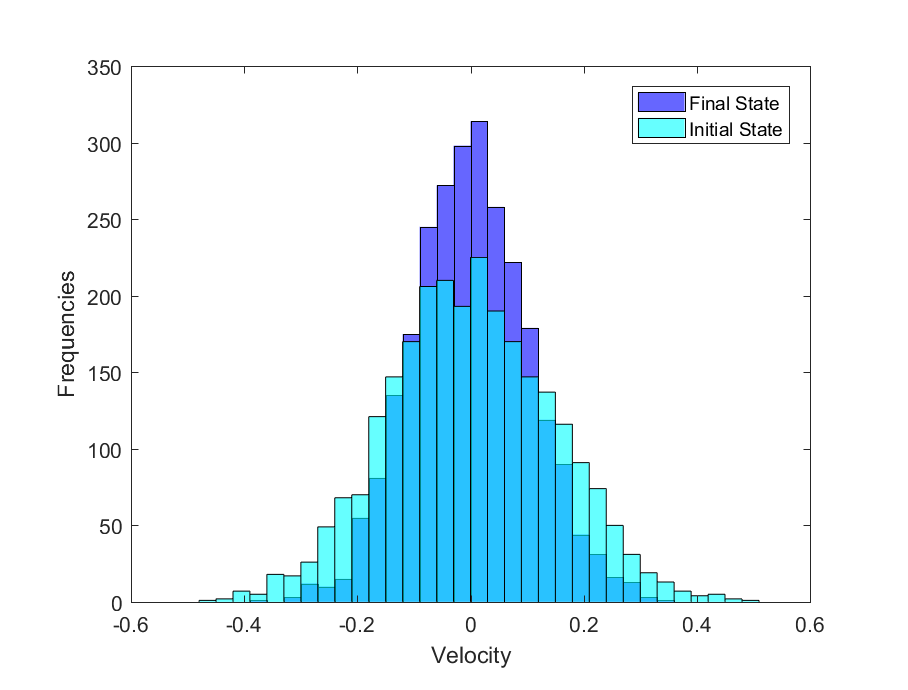
\includegraphics[width=0.5\textwidth]{time_reversible_b0,0g0,50_1000_velocity_histogram.eps} &
    			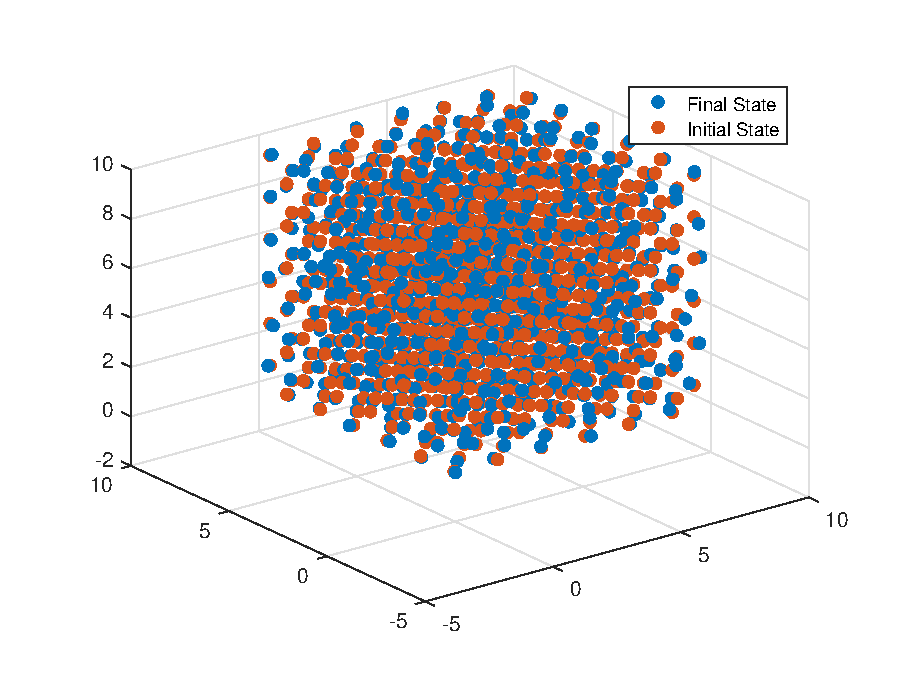
\includegraphics[width=0.5\textwidth]{time_reversible_b0,0g0,50_1000_position_overlay.eps} \\
		\end{tabular}
  		\caption{Changes in position and velocities for $\beta = 0.00$ and $\gamma = 0.50$ after reversing 500 steps}
		\label{fig:time_reversible_b0.00g0.50_1000}
	\end{figure}
}

\only<2-2> {
	\begin{figure}
		\centering
 		\begin{tabular}{@{}cc@{}}
			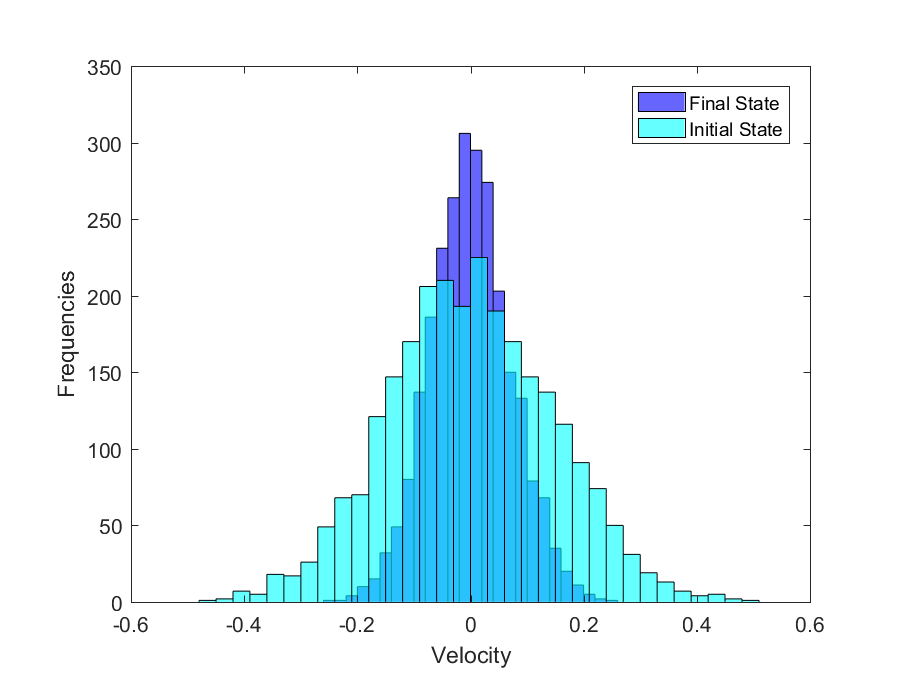
\includegraphics[width=0.5\textwidth]{time_reversible_b0,0g0,75_1000_velocity_histogram.eps} &
    			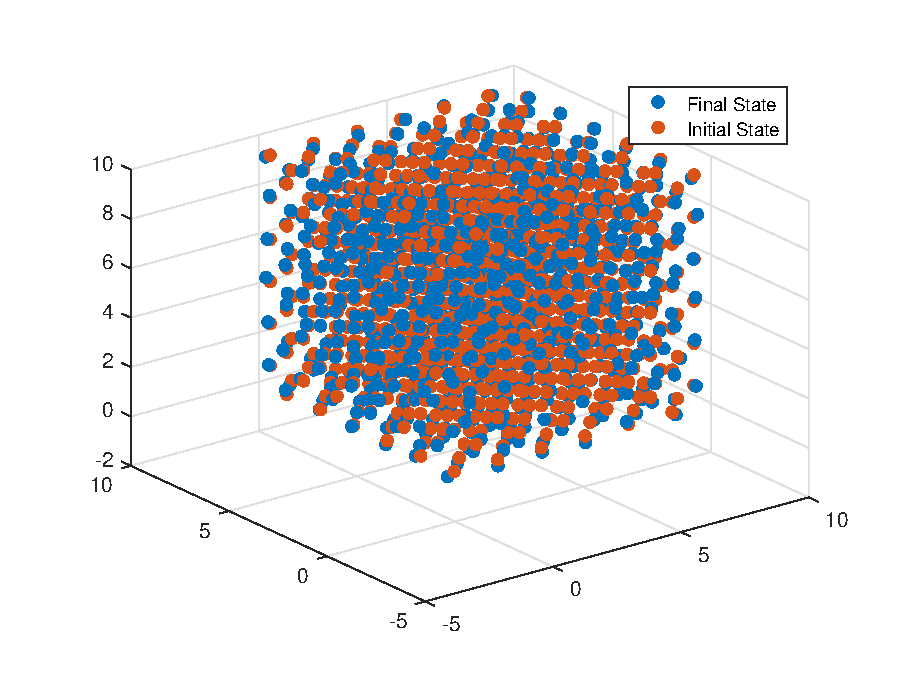
\includegraphics[width=0.5\textwidth]{time_reversible_b0,0g0,75_1000_position_overlay.eps} \\
		\end{tabular}
  		\caption{Changes in position and velocities for $\beta = 0.00$ and $\gamma = 0.75$ after reversing 500 steps}
		\label{fig:time_reversible_b0.00g0.75_1000}
	\end{figure}
}

\only<3-3> {
	\begin{figure}
		\centering
 		\begin{tabular}{@{}cc@{}}
    			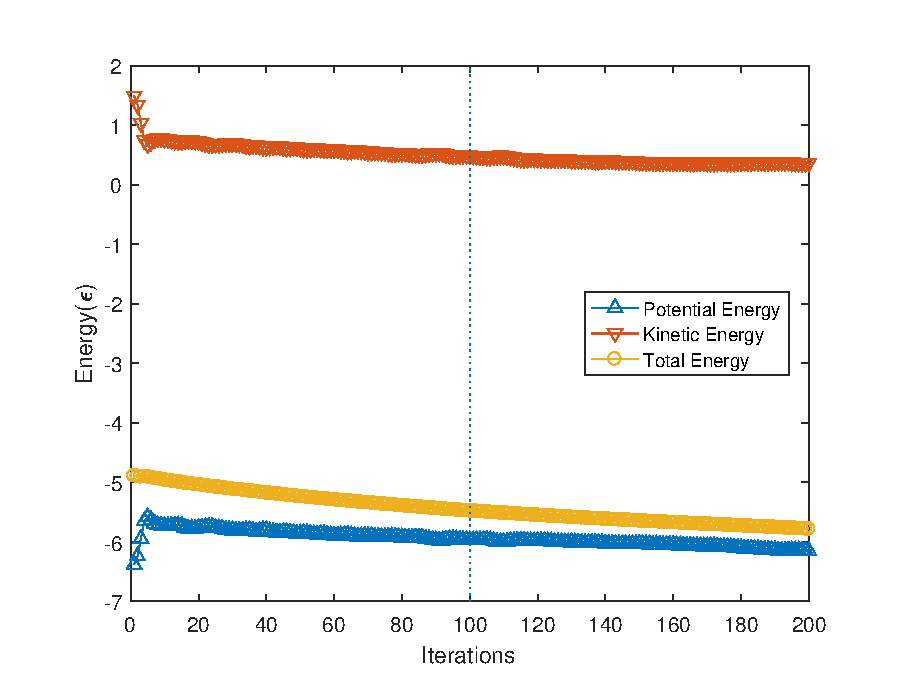
\includegraphics[width=0.5\textwidth]{time_reversible_b0,0g0,75_1000_energy.eps} &
    			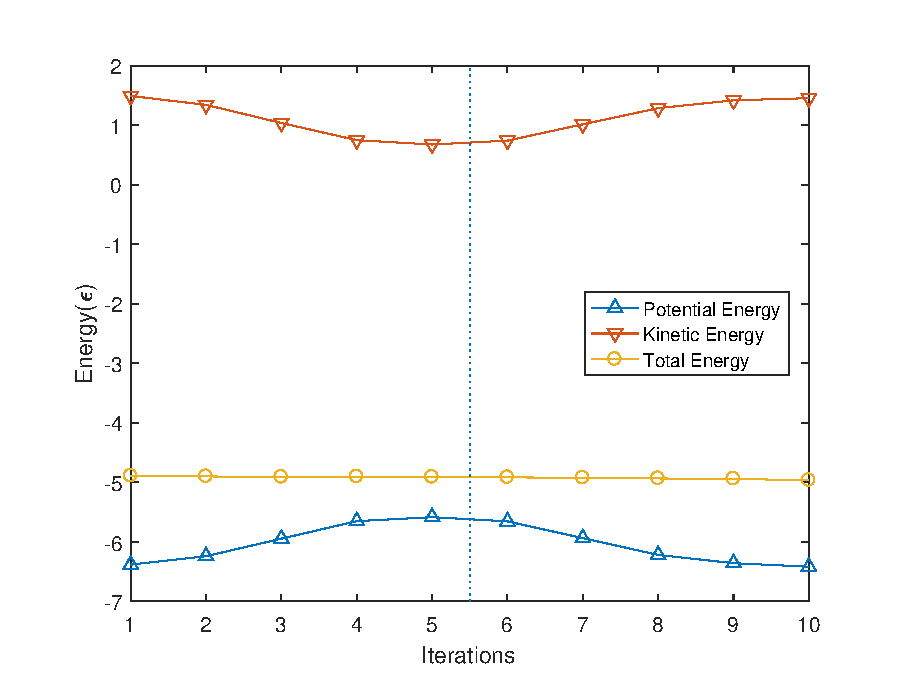
\includegraphics[width=0.5\textwidth]{time_reversible_b0,0g0,75_50_energy.eps} \\
		\end{tabular}
  		\caption{Difference in behaviour of total  energy for $\beta = 0.00$ and $\gamma = 0.75$ over different timesteps}
		\label{fig:time_reversible_b0.00g0.75_1000,50}
	\end{figure}
}

\only<4-4> {
	\begin{figure}
		\centering
 		\begin{tabular}{@{}cc@{}}
    			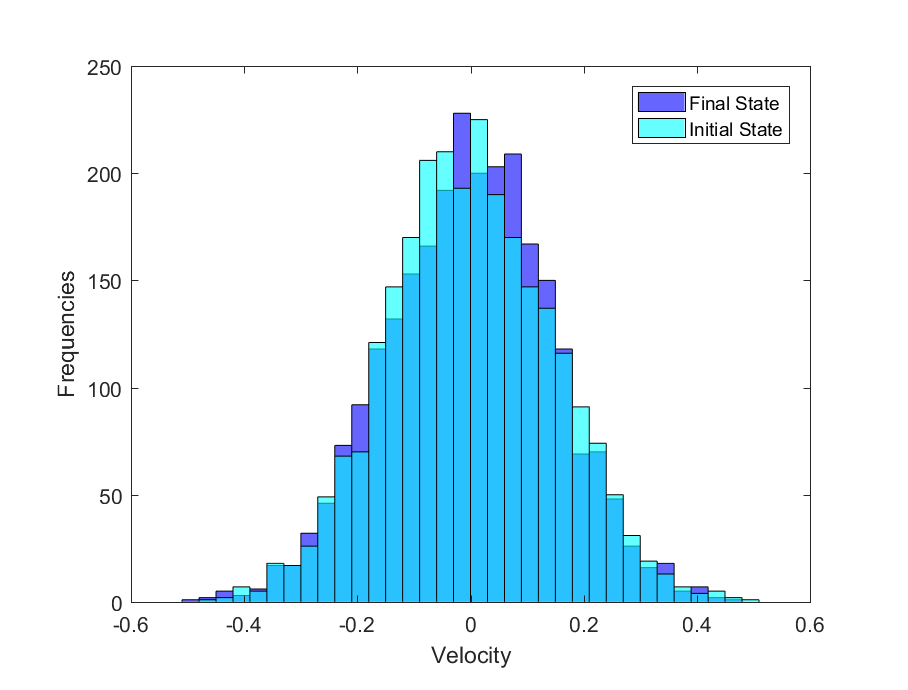
\includegraphics[width=0.5\textwidth]{time_reversible_b0,25g0,50_250_velocity_histogram.eps} &
    			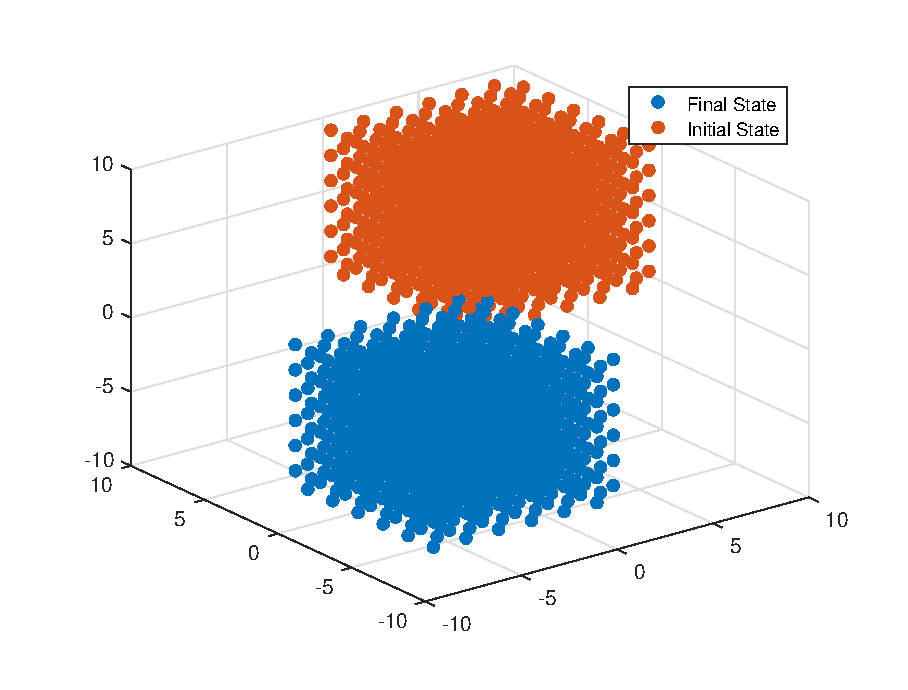
\includegraphics[width=0.5\textwidth]{time_reversible_b0,25g0,50_250_position_overlay.eps} \\
		\end{tabular}
  		\caption{Changes in position and velocities for $\beta = 0.25$ and $\gamma = 0.50$ after reversing 125 steps}
		\label{fig:time_reversible_b0.25g0.50_250}
	\end{figure}
}
\end{frame}

\subsection{Total Angular Momentum}

\begin{frame}{Total Angular Momentum}
\begin{block}{Claim} Angular momentum, $\vec{L} = \sum_{i=1}^{N} \vec{q}_{i} \times \vec{p}_{i}$,  is preserved $\Leftrightarrow \beta = 0, \gamma = \frac{1}{2}$. \end{block}
	\setlength{\belowdisplayskip}{1pt}
\begin{proof}
	\begin{align*}
		\vec{L}_{i+1} - \vec{ L}_{i} &= \sum_{k=1}^{N}\left(\vec{q}_{i+1}\right)_{k} \times \left(\vec{p}_{i+1}\right)_{k} - \sum_{k=1}^{N}\left(\vec{q}_{i}\right)_{k} \times \left(\vec{p}_{i}\right)_{k} \\
		&= h^{2}\left(\gamma - \frac{1}{2}\right)\sum_{k=1}^{N} (\vec{a}_{i})_{k} \times (\vec{p}_{i})_{k} \\ &+ h^{2}\beta\sum_{k=1}^{N} (\vec{a}_{i+1})_{k} \times (\vec{p}_{i+1})_{k} - (\vec{a}_{i})_{k} \times (\vec{p}_{i})_{k} .
	\end{align*}
	So $\vec{L}_{i+1}-\vec{L}_{i} = 0 \Leftrightarrow \beta = 0, \gamma = \frac{1}{2}$.
\end{proof}
\end{frame}

\begin{frame}{Total Angular Momentum}
\begin{table}
	\centering
	\begin{tabular}{ |r|r|r|r| }
		\hline
		Iteration & x-component & y-component & z-component\\
		\hline
		10 & 493.28 & -402.32 & 1407.30 \\
		20 & -4.80 & -10.18 & 914.24 \\
		30 & 320.20 & -147.35 & 980.93 \\
		40 & 717.70 & -181.21 & 704.27 \\
		50 & 594.66 & 152.47 & 507.19 \\
		\hline
	\end{tabular}
	\caption{Total angular momentum of the system with $\beta = 0, \gamma = \frac{1}{2}$ over the first 50 iterations}
	\label{tbl:total_angular_momentum_50_iterations}
\end{table}
\end{frame}

\subsection{Total Energy}
\begin{frame}{Recap: Physical Interpretation of $\gamma$}
\begin{itemize}
	\item
	$\gamma$ plays the role of a damping factor in the energy of the system.
	\item
	The energy of the system is damped by a factor of $\gamma - \frac{1}{2}$.
	\item
	If $\gamma > \frac{1}{2}$, the energy is damped.
	\item
	If $\gamma < \frac{1}{2}$, the energy grows.
\end{itemize}
\end{frame}

\begin{frame}{Total Energy - Implicit Methods}
We start by quoting Simo, Tarnow, and Wong: \\
``\textit{What may seem surprising is that all of the implicit members of the Newmark family, perhaps the most widely used time-stepping algorithms in nonlinear structural dynamics, are not designed to conserve energy and also fail to conserve momentum.}''
\end{frame}

\begin{frame}{Total Energy - Implicit Methods}
\only<1-1> {
		\centering
		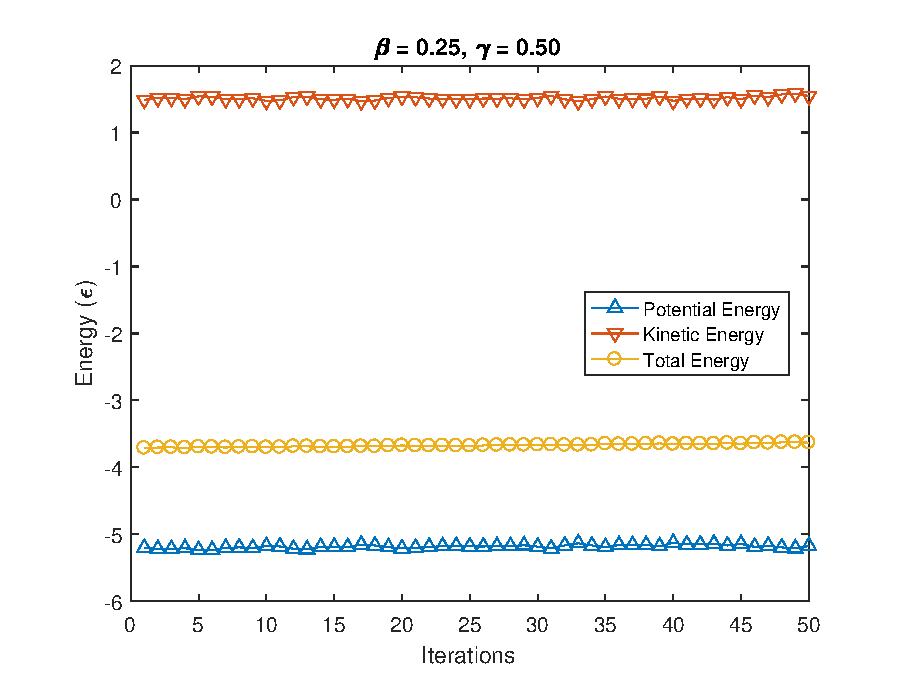
\includegraphics[scale=0.60]{energy_b0,25_g0,50_long.eps}
}

\only<2-2> {
		\centering
		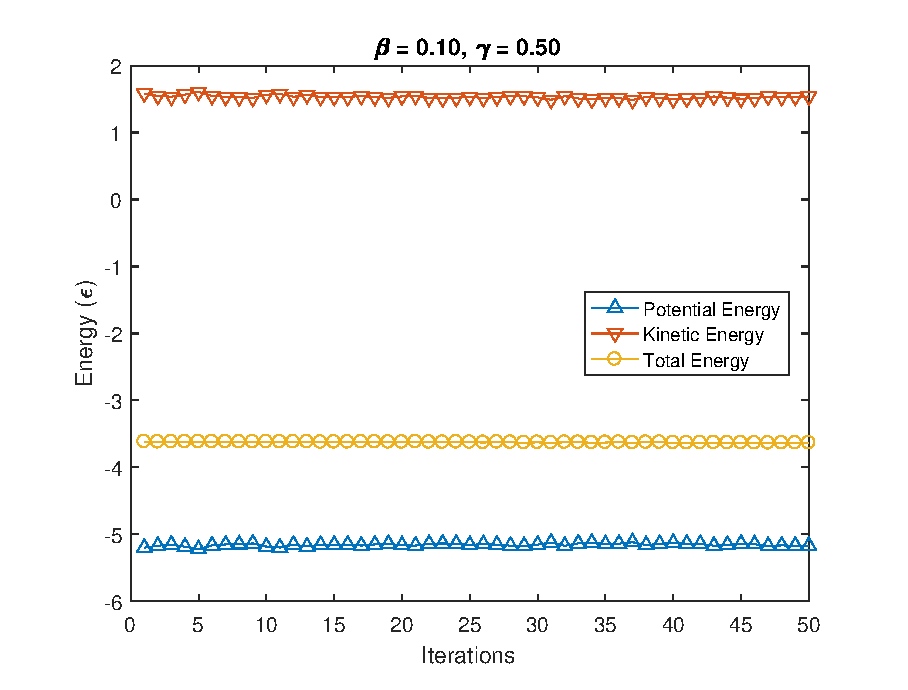
\includegraphics[scale=0.60]{energy_b0,10_g0,50_long.eps}
}

\only<3-3> {
		\centering
		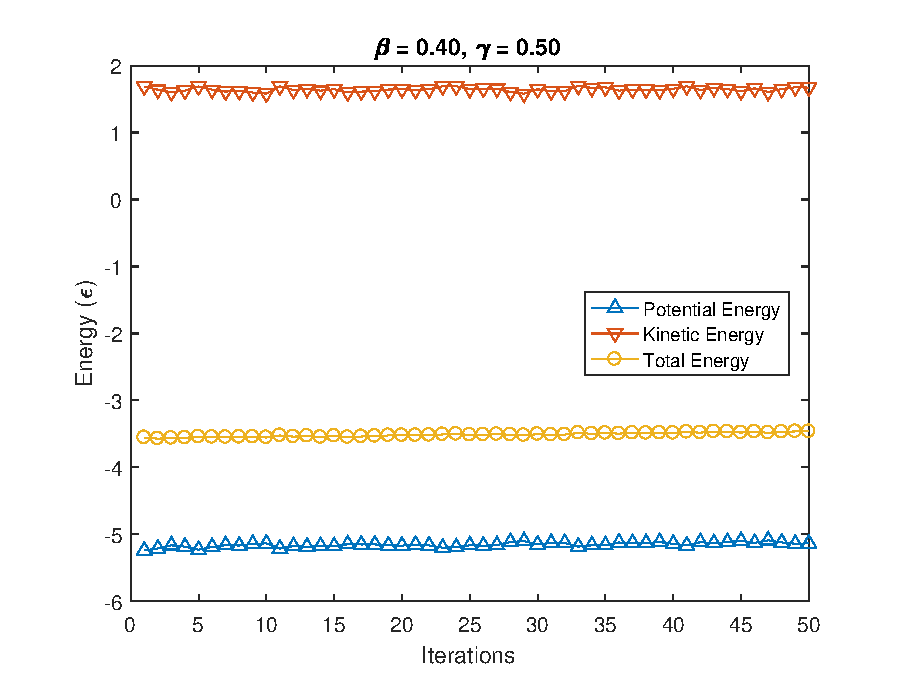
\includegraphics[scale=0.60]{energy_b0,40_g0,50_long.eps}
}
\end{frame}

\section{Conclusion}

\begin{frame}{Conclusion}

\end{frame}

\end{document}